\documentclass[aspectratio=169]{beamer}

\usepackage{mystyle}

\title{Measuring the Information Content of VIX Volatility}
\author{Context: Humboldt Project\\
Supervisor: Prof. Franziska Peter\\
Author: Sophia Gläser (7. Semester BA CME)}
\date{\small \today}

\addbibresource{./bib/bibliography.bib} 

\begin{document}

\begin{frame}
\maketitle
\end{frame}

\begin{frame}
\frametitle{Table of Contents}
\tableofcontents
\end{frame}

\section{Introduction}

\begin{frame}
\frametitle{Motivation: Why this project? Why does Volatility matter?}
	\begin{itemize}
	\item For the stability of the financial system, precise risk measurement is of great importance
		\begin{itemize}
		\item Volatility is closely related to risk 
		\item Volatility is crucial input to risk measures, such as the Value at Risk\footnote{The Value at Risk is a quantile of the loss function, used for example by banks to estimate the amount of assets needed to cover possible losses. It estimates which loss is not going to be exceeded in a given time interval, for a given probability}
		\end{itemize}
	\item Moreover volatility is used for..
		\begin{itemize}
		\item .. the pricing of financial instruments, such as derivatives
		\item .. the risk-return trade-off and therefore management decisions
		\end{itemize}
	\item Finally, a good volatility estimate might be a valuable starting point for a forecast
	\end{itemize}
\end{frame}

\begin{frame}
\frametitle{More closely: What exactly is Volatility?}
	\begin{itemize}
	\item In Finance, we are usually interested in the \textit{conditional} standard deviation from the expected value of the underlying asset return \parencite{tsay2005}
	\item What causes asset price movement and thus volatility?
		\begin{itemize}
		\item Assuming Market efficiency (as introduced by \citeauthor{fama1970}), stock prices incorporate all available information from the market, because of competition and free entry 
		\item But that does not does not give us information about the volatility of stock prices
		\end{itemize}
	\end{itemize}
\end{frame}

\begin{frame}
\frametitle{The Problem: Why is it so hard to measure and forecast volatility?}
	\begin{itemize}
	\item Volatility is not directly observable
		\begin{itemize}
		\item We can estimate it for a given time period 
		\item However, stock volatility consists of intraday and overnight volatility, each containing different information
		\end{itemize}
	\item We can however observe some characteristics of volatility (stylized facts), such as
		\begin{itemize}
		\item volatility clustering (periods of high volatility are followed by periods of high volatility, and similar for low volatility)
		\item volatility is often stationary (it varies only within a fixed range)
		\item leverage effect: volatility reacts differently to price drop or increase
		\end{itemize}
	\end{itemize}
\end{frame}

\begin{frame}
\frametitle{Maybe a solution: How volatility has been calculated so far}
	\begin{itemize}
	\item According to this stylized facts, we can use (econmetric) models that best capture the characteristics of volatility
	\item There is however multiple approaches to model volatility, examples are
		\begin{itemize}
		\item Econometric models using historic volatility (e.g. ARCH)
		\item Black-and-Scholes implied volatility
		\end{itemize}
	\item Many papers argue, that Black-and Scholes implied volatility contains significant information for realized volatility \parencite{jiang2005}
	\end{itemize}
\end{frame}

\begin{frame}
\frametitle{Maybe a solution: Black-and-Scholes implied volatility}
%
	\begin{itemize}
	\item Intuition behind Black-and-Scholes (BS) implied volatility
		\begin{itemize}
		\item The BS model is an option pricng model, that uses volatility as an input
		\pro By using option prices from the market, it is possible to turn the calculation around and derive an \textit{option implied volatility}
		\pro as options are contracts to buy an underlying in the future, then contain the market's expectation of future stock price movement 
		\end{itemize}
	%
	\item There are however some problems with the BS implied volatility
		\begin{itemize}
		\con The Black-and-Scholes model is mainly based on at-the-money options 
		\con Most importantly The Black-and-Scholes model makes an assumption about how the prices are formed (pricing assumption), and assumes that stock prices follow geometric Brownian motion)
		\end{itemize}
	%
\setbeamertemplate{itemize item}[compoundarrow]
	\item Joint hypothesis problem: Testing for BS implied volatility is always a test of \textit{both} market effi	ciency and the BS pricing assumptions
	\end{itemize}
\end{frame}

\begin{frame}
\frametitle{Solving the joint hypothesis problem: Model-free implied volatility}
	\begin{itemize}
	\item For model-free implied volatility, no assumption is made regarding the underlying stochastic process, and it is not based on any particular option pricing model
		\begin{itemize}
		\pro The VIX includes information from both at-the-money and out-of-money options
		\pro As no pricing assumption is made, the model-free implied volatility provides a direct test of the informational efficiency of the options market
		\item 
		\end{itemize}
	\item One of the fist model-free implied volatility indices was the VIX from CBOE \parencite{exchange2009}
		\begin{itemize}
		\item VIX measures the market's expectation of 30-day volatility
		\end{itemize}
	\end{itemize}
\end{frame}

\section{Data}

\begin{frame}
\frametitle{Volatility of S\&P 500}
	\begin{itemize}
	\item Components of Dataset
		\begin{itemize}
		\item VIX, downloaded from CBOE
		\item Realized Volatility, downloaded from Oxford Man Institute
		\item S\&P 500, downloaded from CBOE
		\end{itemize}
	\item Sampling period January 2000 - December 2017
	\end{itemize}
\end{frame}

\begin{frame}
\frametitle{S\&P 500 in Comparison to VIX}
	\begin{figure}
	\centering
	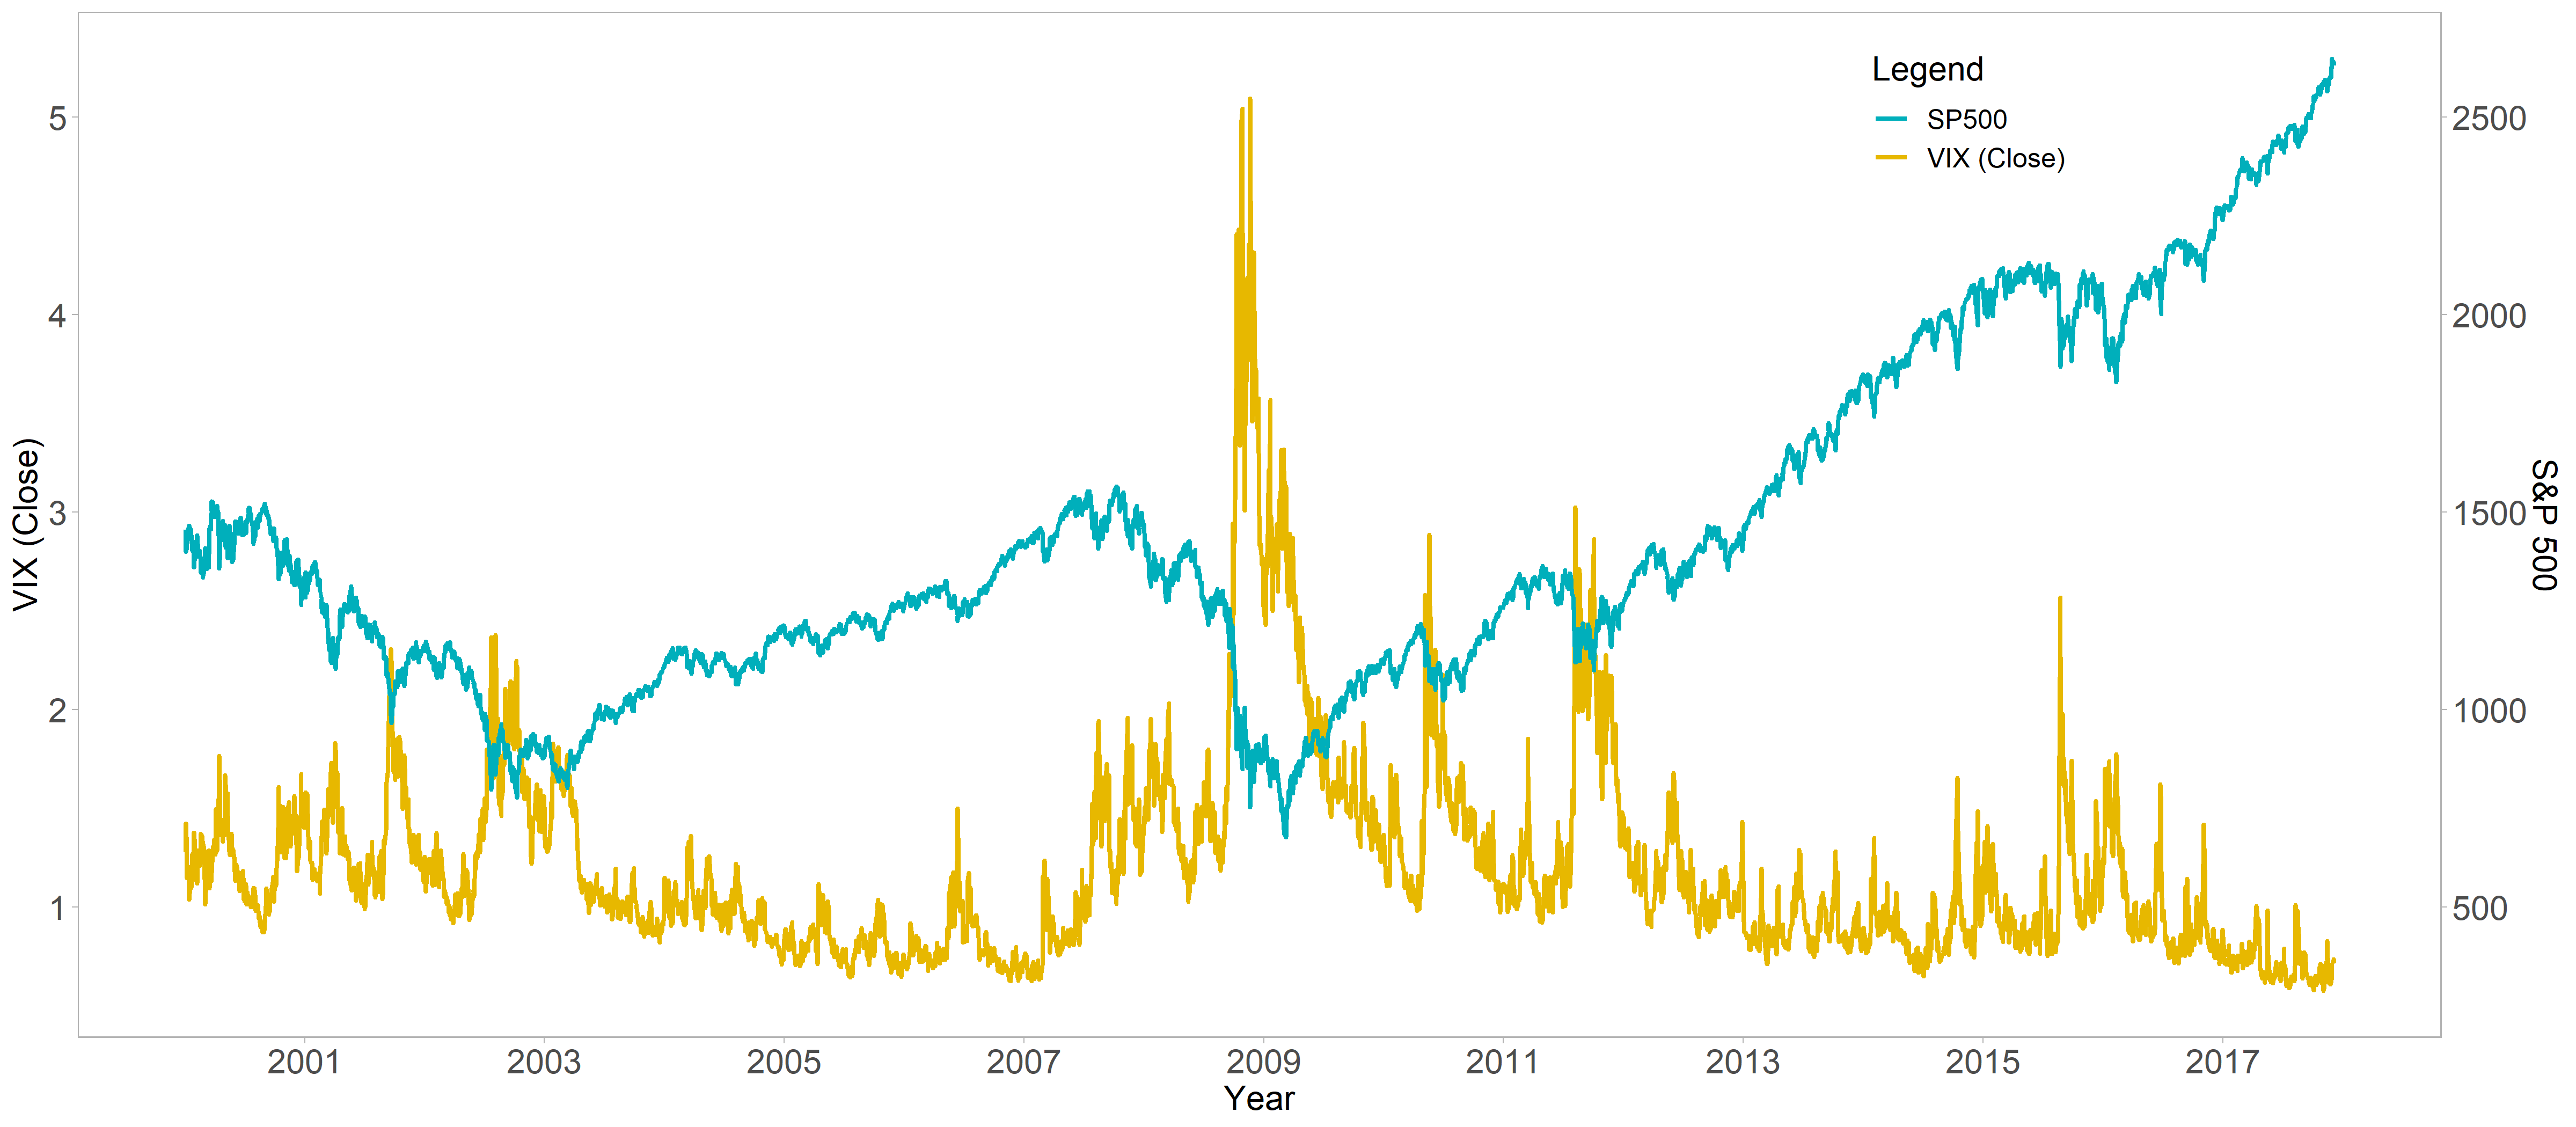
\includegraphics[scale = 0.35]{graphics/SPandViX.png}
	\end{figure}
\end{frame}

\begin{frame}
\frametitle{S\&P 500 in Comparison to VIX and Realized Volatility}
	\begin{figure}
	\centering
	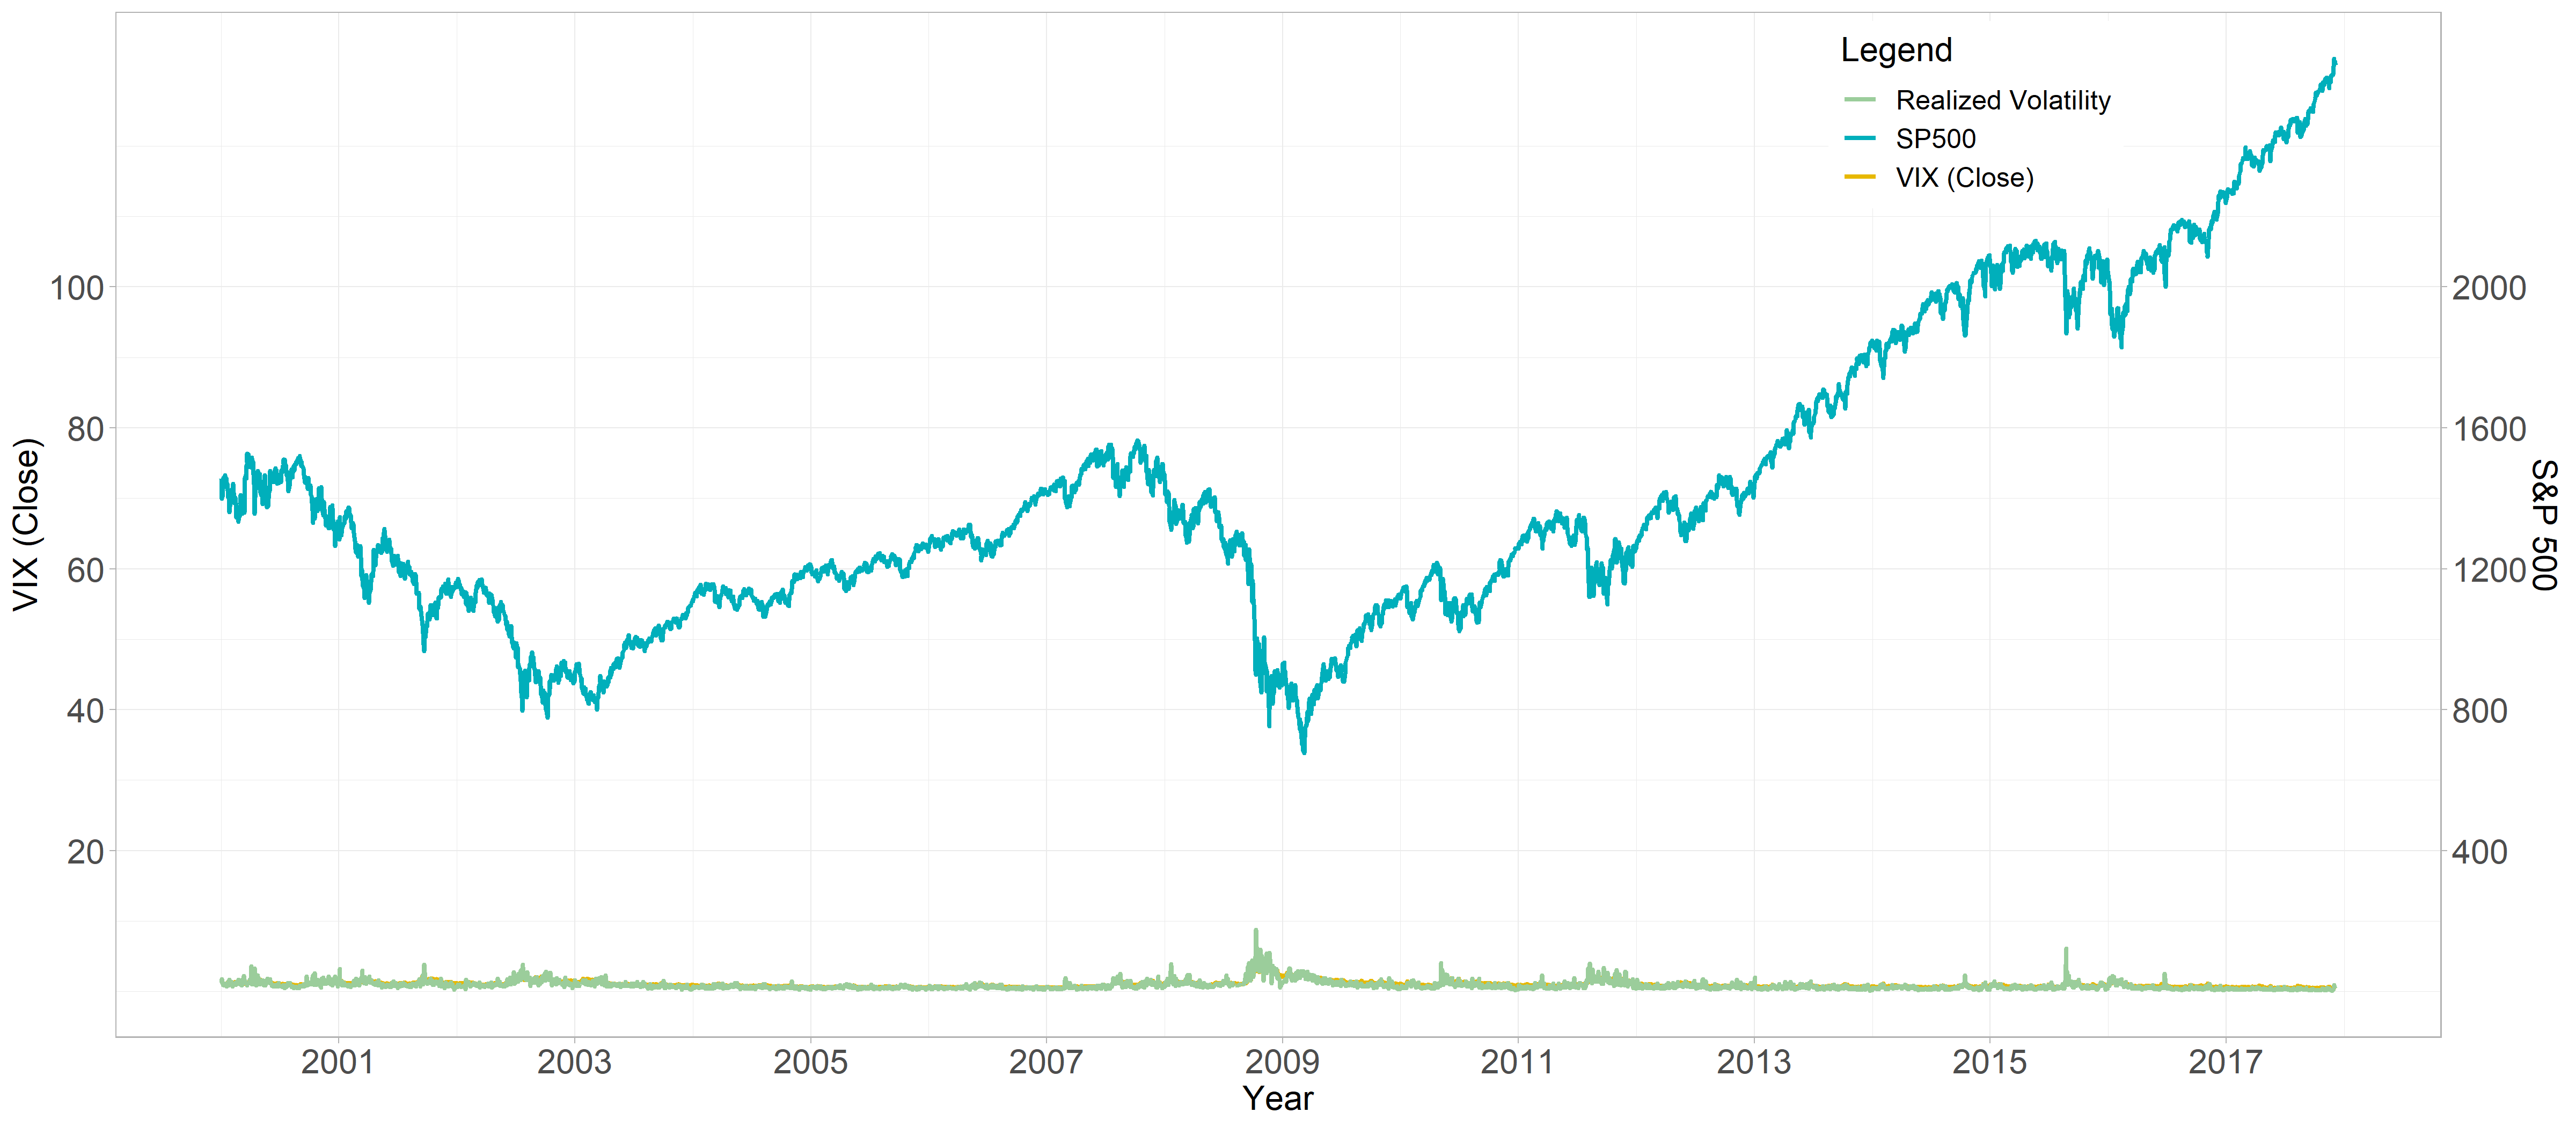
\includegraphics[scale = 0.35]{graphics/SPandVolandViX.png}
	\end{figure}
\end{frame}

\section{Method}


\begin{frame}
\frametitle{My Method: Regression and HAR Model}
%
Stepwise regressions, to compare information content:
	\begin{equation}
	\sigma_{t+1} = c + \beta^{d} RV^{d}_{t-1} + \beta^{w} RV^{w}_{t-1} + \beta^{m} RV^{m}_{t} 
	\end{equation}	
	\begin{equation}
	\sigma_{t+1} = c + \beta^{d} RV^{d}_{t-1} + \beta^{w} RV^{w}_{t-1} + \beta^{m} RV^{m}_{t} + \beta^{m} VIX^{m}_{t}
	\end{equation}
$+$ the same regressions as log-log model\\
with the weekly aggregation period being (monthly similar with 20 days):
	\begin{equation*}
	\sigma^{w}_{t} = \frac{1}{5} (RV^{d}_{t} + RV^{d}_{t-1d} + RV^{d}_{t-2d} + RV^{d}_{t-3d} + RV^{d}_{t-4d})
	\end{equation*}
and Realized Variance (RV) being: $	RV^{d}_{t} = \sqrt[]{\sum_{m=1}^{M} r^{2}_{t,m}} $\\
%
\begin{footnotesize}
$\sigma$ = Volatility (sd), $RV$ = Realized Variance with M equally spaced intraday returns for a day t, with m = 1,..,M, here 10min returns
\end{footnotesize}
%
\end{frame}

\begin{frame}
\frametitle{My Method: Regression and HAR Model}
HAR-RV Model (not implemented yet)
\begin{equation}
	\sigma_{t+1} = c + \beta^{d} RV^{d}_{t-1} + \beta^{w} RV^{w}_{t-1} + \beta^{m} RV^{m}_{t} + \tilde{w^{d}_{t+1d}}
	\end{equation}	
	\begin{equation}
	\sigma_{t+1} = c + \beta^{d} RV^{d}_{t-1} + \beta^{w} RV^{w}_{t-1} + \beta^{m} RV^{m}_{t} + \beta^{m} VIX^{m}_{t} + \tilde{w}^{d}_{t+1d}
	\end{equation}
\begin{footnotesize}
$\tilde{w}^{d}_{t+1d}$ = innovation
\end{footnotesize}

\end{frame}


\section{Results so far}

\begin{frame}
\frametitle{Regression Results}
\begin{scriptsize}
\begin{minipage}{0.45\textwidth}
	\begin{figure}[!htbp]
	\caption{level-level Model}
	\centering
	
\begin{tabular}{l c c }
\hline
 & HAR-RV & HAR-RV with VIX \\
\hline
Intercept    & $0.00^{**}$  & $-0.00^{***}$ \\
             & $(0.00)$     & $(0.00)$      \\
$RV_{t}^{d}$ & $0.26^{***}$ & $0.22^{***}$  \\
             & $(0.02)$     & $(0.02)$      \\
$RV_{t}^{w}$ & $0.40^{***}$ & $0.38^{***}$  \\
             & $(0.03)$     & $(0.03)$      \\
$RV_{t}^{m}$ & $0.26^{***}$ & $0.06$        \\
             & $(0.03)$     & $(0.03)$      \\
VIX          &              & $0.00^{***}$  \\
             &              & $(0.00)$      \\
\hline
R$^2$        & 0.55         & 0.56          \\
Adj. R$^2$   & 0.55         & 0.56          \\
Num. obs.    & 4272         & 4272          \\
RMSE         & 0.00         & 0.00          \\
\hline
\multicolumn{3}{l}{\scriptsize{$^{***}p<0.001$, $^{**}p<0.01$, $^*p<0.05$}}
\end{tabular}

	\end{figure}
\end{minipage}
%
\begin{minipage}{0.45\textwidth}
	\begin{figure}[!htbp]
	\caption{log-log Model}
	\centering
	
\begin{tabular}{l c c }
\hline
 & Historic & Historic and VIX \\
\hline
Intercept    & $0.19^{***}$ & $2.68^{***}$  \\
             & $(0.04)$     & $(0.10)$      \\
$RV_{t}^{d}$ & $0.34^{***}$ & $0.24^{***}$  \\
             & $(0.02)$     & $(0.02)$      \\
$RV_{t}^{w}$ & $0.41^{***}$ & $0.28^{***}$  \\
             & $(0.03)$     & $(0.03)$      \\
$RV_{t}^{m}$ & $0.20^{***}$ & $-0.13^{***}$ \\
             & $(0.02)$     & $(0.02)$      \\
VIX          &              & $0.80^{***}$  \\
             &              & $(0.03)$      \\
\hline
R$^2$        & 0.73         & 0.77          \\
Adj. R$^2$   & 0.73         & 0.77          \\
Num. obs.    & 4435         & 4435          \\
RMSE         & 0.30         & 0.28          \\
\hline
\multicolumn{3}{l}{\scriptsize{$^{***}p<0.001$, $^{**}p<0.01$, $^*p<0.05$}}
\end{tabular}

	\end{figure}
\end{minipage}
\end{scriptsize}
\end{frame}


\section{Possible Problems coming up}

\begin{frame}
\frametitle{Questions currently to solve}
	\begin{itemize}
	\item Having gathered all this information about volatility measurement, what is the most accurate way to set up my regressions and my HAR-RV model?
	
	\end{itemize}
\end{frame}

%\section*{Sources}

\begin{frame}
\printbibliography
\end{frame}

\section{Appendix}
\begin{frame}
\frametitle{The Black and Scholes Equation}
%
\begin{minipage}{0.6\textwidth}
\begin{small}
%
price of an option over time:
\begin{equation}
	\frac{\partial \mathrm C}{ \partial \mathrm t } + \frac{1}{2}\sigma^{2} \mathrm S^{2} \frac{\partial^{2} \mathrm C}{\partial \mathrm C^2}
	+ \mathrm r \mathrm S \frac{\partial \mathrm C}{\partial \mathrm S}\ =
	\mathrm r \mathrm C 
	\label{eq:1}
\end{equation}
%
calculate the price of European call and put option: 
\begin{equation}
	\mathrm C(\mathrm S,\mathrm t)= \mathrm N(\mathrm d_1)\mathrm S - \mathrm N(\mathrm d_2) \mathrm K \mathrm e^{-rt}
	\label{eq:2}
\end{equation}
\vspace{-3pt}
%
\begin{equation}
	\mathrm d_1= \frac{1}{\sigma \sqrt{\mathrm t}} \left[\ln{\left(\frac{S}{K}\right)} + t\left(r + \frac{\sigma^2}{2} \right) \right]
\end{equation}
\vspace{-3pt}
%
\begin{equation}
	\mathrm d_2= \frac{1}{\sigma \sqrt{\mathrm t}} \left[\ln{\left(\frac{S}{K}\right)} + t\left(r - \frac{\sigma^2}{2} \right) \right]
\end{equation}
\vspace{-3pt}
%
\begin{equation}
	N(x)=\frac{1}{\sqrt{2\pi}} \int_{-\infty}^{x} \mathrm e^{-\frac{1}{2}z^2} dz
	\label{eq:5}
\end{equation}
\end{small}
\end{minipage}
%
\begin{minipage}{0.35\textwidth}
\begin{footnotesize}
\begin{itemize}
	\item[] C = Call option price 
	\item[] S = Current stock price
	\item[] K = Strike price of the option
	\item[] r = risk-free interest rate (a number between 0 and 1)
	\item[] $\sigma$ = volatility of the stocks return (a number between 0 and 1)
	\item[] t = time to option maturity (in years)
	\item[] N = normal cumulative distribution function
\end{itemize}
\end{footnotesize}
\end{minipage}
%
\end{frame}

\begin{frame}
\frametitle{The VIX Equation}
	\begin{equation}
	\sigma^{2} = \frac{2}{T} \sum_{i} \frac{\Delta K_{i}}{K_{i}^{2}} e^{RT} Q(K_{i}) - \frac{1}{T} (\frac{F}{K_{0}} - 1)^{2}
	\end{equation}
\end{frame}


\end{document}
